\section{Programming Model}

\begin{figure}

  \begin{ocaml}
  module type DALI = sig
    type 'a 'b t
    val return : 'b -> 'a 'b t
    val bind : 'a 'b t -> ('b -> 'a 'c t) -> 'a 'c t
    val get_current_version: unit -> 'a 'a t
    val with_init_version_do: 'a -> 'a 'b t -> 'b
    val fork_version : 'a 'b t -> 'a unit t
    val sync_next_version: unit -> ?v:'a -> 'a 'a t
  end
  \end{ocaml}

\label{fig:dali-monad}
\caption{Signature of the \name monad}
\end{figure}

\begin{figure}

  \begin{ocaml}
  module type CANVAS = sig
    type pixel = {r:char; g:char; b:char}
    type tree = 
      | N of pixel
      | B of {tl: tree; tr: tree; bl: tree; br: tree} 
    type t = {max_x:int; max_y:int; canvas:tree} [@@deriving versioned]
    type loc = {x:int; y:int}
  
    val new_canvas: int -> int -> t
    val set_px: t -> loc -> pixel -> t
    val get_px: t -> loc -> pixel
    val merge: (* lca *)t -> (* v1 *)t -> (* v2 *)t -> t
  end
  \end{ocaml}

\label{fig:canvas-sig}
\caption{\drawsome: a sample \name application}
\end{figure}

In this section, we describe the \name programming model through the
example of a collaborative drawing application we call \drawsome.

Fig.~\ref{canvas-sig} shows the signature of the \drawsome
application. \drawsome represents a free-hand drawing canvas as a tree
of quadrants, where each quadrant is simply a leaf node unless it has
pixels of different colors. Quadrants are expanded into a tree
structures as an when pixels are colored (the color scheme used is
rgb). The representation is thus optimized for sparse canvases, such
as whiteboards. The application supports three simple operations:
creating a new canvas, setting the pixel at a specified coordinate,
and returning the pixel at a given coordinate. The \C{merge} function
and \C{deriving versioned} directive are explained below.

\begin{figure}
\centering
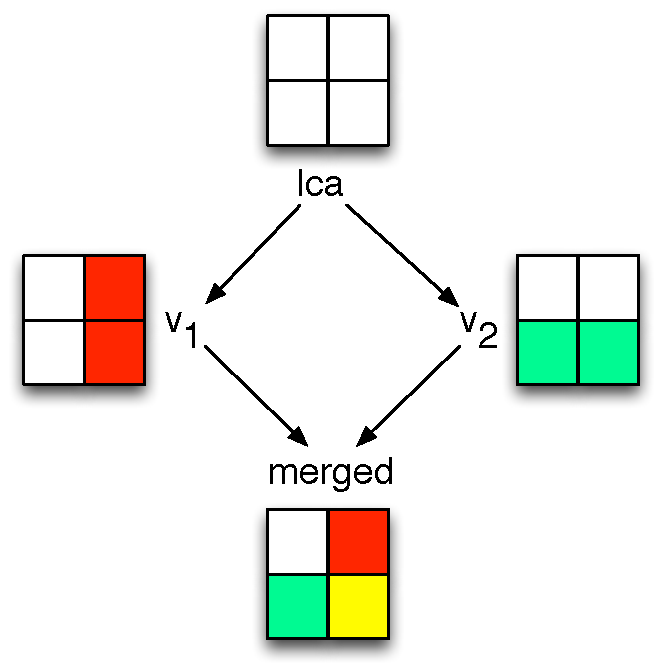
\includegraphics[scale=0.5]{Figures/canvas-merging}

\caption{Merging concurrent versions (\C{v1} and \C{v2} ) of a drawing
canvas. \C{lca} is their common ancestor.}
\label{fig:canvas-merging}
\end{figure}

\drawsome lets multiple users collaborate on a canvas that is
conceptually shared among all the collaborators. Under a shared-memory
abstraction, there would be a single copy of the canvas that is
updated concurrently by multiple clients such that from the
perspective of any single client, the canvas would change without any
explicit intervention. \name ascribes functional semantics to sharing
by letting each client work on its own version of the state (a data
structure), and later merging the concurrent versions on-demand. Thus,
the primary artifact of the \name programming model is a versioned
data structure. The library operates on a representation of versioned
data structures optimized for persistence on disk
(Sec.~\ref{sec:persistence}). \name's meta-programming component
automatically synthesizes this representation, along with the
functions that translate between representations, for the data type
definitions marked with the ppx~\cite{ppx} directive \C{deriving
versioned}. Concretely, for the \C{Canvas} module, \name synthesizes
a \C{Canvas.Versioned} module with a type \C{t}, and functions
\C{of\_canvas} and \C{to\_canvas} of types \C{Canvas.t $\rightarrow$
t} and \C{t $\rightarrow$ Canvas.t}, respectively.

\name requires a three-way \C{merge} function to merge the concurrent
versions of a drawing canvas. The three arguments include two
concurrent versions (\C{v1} and \C{v2}), and their least common
ancestor (\C{lca}) - the version from which the two concurrent
versions evolved independently. The merge function can make use of the
pixel values of the common ancestor to merge the pixel values on both
the canvases. For instance, if the color of a pixel in \C{v1} is white,
and in \C{v2} it is green, and its color in \C{lca} is
white, then it means that only \C{v2} modified the color. Hence the
pixel is colored green in the merged canvas. On the other hand, if the
pixel is red in \C{v1}, then it means that both
\C{v1} and \C{v2} have modified the color. In such case, an appopriate
color-mixing algorithm can be used to determine the color of pixel.
For instance, the pixel can be colored yellow - an additive
combination of red and green. The logic is illustrated in
Fig.~\ref{fig:canvas-merging}.

The \name programming model lets programmers define and compose
concurrent computations around versioned data structures.
Fig.~\ref{fig:dali-monad} shows the signature of the \name module that
implements the programming model along the lines of the well-known
\C{State} monad~\cite{wadler-monad}. The monad encapsulates a
versioned functional state (\C{'a}) and the type \C{'a 'b t}
represents a monadic computation that returns a \C{'b} result.
Functions \C{return} and \C{bind} have their usual monadic
interpretation. \C{get\_current\_version} is like the \C{State}
monad's \C{get}; it returns the versioned state encapsulated by the
monad. \C{with\_init\_version\_do} runs a monadic computation against
a given initial version and returns the result. \C{fork\_version}
returns a computation that forks a new concurrent version from the
current version, and runs the given monadic computation asynchronously
against the forked version.  The semantics of \C{sync\_next\_version}
(simply called \C{sync}) is somewhat involved: the function accepts
a \emph{proposal} for the next version of the
state, where \C{next} is defined w.r.t the current version, and
returns (via a monad) the actual next version, which becomes the
current version for rest of the computation.  The next version is
created by merging the proposal with a subset of concurrent versions
that became available since the last merge or fork. Thus, \C{sync}
effectively lets a computation sync with a subset of concurrent
computations and obtain their latest updates.

\begin{figure}
\centering
\begin{tabular}{l||l||l}
\begin{ocaml}
let alice_f : C.t unit t = 
  get () >>= fun c0 -> 
  fork bob_f >>= fun () ->
  let c0' = C.draw_line c0 
    {x=0;y=0}
    {x=4;y=0} in
  sync () ~v:c0' >>= 
  fun c1 ->
  let c1' = C.draw_line c1 
    {x=0;y=4} 
    {x=4;y=4} in
  sync () ~v:c1' >>= 
  fun c2 -> return ()
\end{ocaml}
&
\begin{ocaml}
let bob_f : C.t unit t = 
  get () >>= fun c0 -> 
  fork cheryl_f >>= 
  fun () ->
  let c0' = C.draw_line c0 
    {x=0;y=0} 
    {x=0;y=4} in
  sync () ~v:c0' >>= 
  fun c1 -> sync () >>= 
  fun c2 -> return ()
\end{ocaml}
&
\begin{ocaml}
let cheryl_f : C.t unit t = 
  get () >>= fun c0 -> 
  let c0' = C.draw_line c0 
    {x=4;y=0} 
    {x=4;y=0} in
  sync () ~v:c0' >>= 
  fun c1 -> sync () >>= 
  fun c2 -> return ()
\end{ocaml}
\\
\end{tabular}
\caption{\drawsome: A collaborative drawing session between Alice,
Bob, and Cheryl}
\label{fig:canvas-sessions-code}
\end{figure}

\begin{figure}
\centering
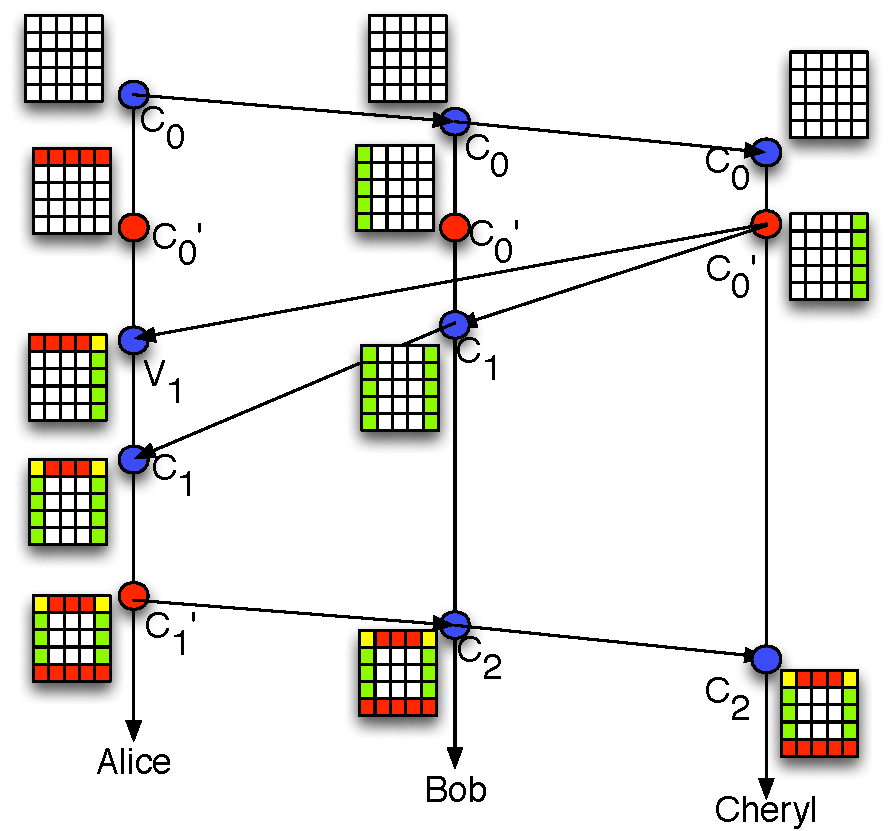
\includegraphics[scale=0.6]{Figures/canvas-sessions}

\caption{\drawsome: Collaborative drawing session visualized}
\label{fig:canvas-sessions}
\end{figure}

Fig.~\ref{fig:canvas-sessions-code} demonstrates how a collaborative
drawing session between Alice, Bob and Cheryl can be composed using
\name. A possible execution of the session is visualized in
Fig.~\ref{fig:canvas-sessions}. Assume that the session starts with
Alice on a $5\times 5$ blank canvas, as shown below:
\begin{ocaml}
  module C = Canvas;; open Dali;;
  with_init_version_do (C.new_blank 5 5) alice_f 
\end{ocaml}
Alice starts by reading the current version of the canvas, which is
blank. She then invites Bob for collaboration by forking a new
concurrent version for Bob. Bob in turn invites Cheryl for
collaboration. All three of them start working on the blank canvas.
Alice draws a red horizontal line from $(0,0)$ (top-left) to $(4,0)$
(top-right) using \C{C.draw\_line} (definition not shown; can be
constructed using \C{set\_px}). Meanwhile, Bob draws a green vertical
line from $(0,0)$ to $(0,4)$, and Cheryl draws a similar line from
$(4,0)$ to $(4,4)$. All three of them call \C{sync} with their
respective proposals ($C_0'$). While any partial ordering of
concurrent \C{syncs} is valid, we consider a linear order where
Cheryl's \C{sync} happens first, followed by Bob's and then Alice's.
Cheryl's \C{sync} does not find any concurrent versions, hence
installs the proposed version ($C_0'$) as the next version on Cheryl's
branch. Bob's \C{sync} finds Cheryl's $C_0'$ as a concurrent version,
and merges it with its proposal to produce the next version $C_1$,
which is installed on Bob's branch.  and returned by \C{sync} (\C{c1}
in second column of Fig.~\ref{fig:canvas-sessions-code}). The least common
ancestor (LCA) for this merge is the initial version ($C_0$), and the two
concurrent versions are Bob's $C_0'$ and Cheryl's $C_0'$. Next,
Alice's \C{sync} finds Cheryl's $C_0'$ and Bob's $C_1$ as concurrent
versions, and merges them successively with Alice's proposal. For the
first merge, the two concurrent versions are Alice's $C_0'$ and
Cheryl's $C_0'$, and the LCA is the initial version
($C_0$). The result of this merge is installed as the next version
($\C{C_0''}$) on Alice's branch. For the next merge, the two
concurrent versions are Alice's $C_0''$ and Bob's $C_1$ and the LCA is
Cheryl's $C_0'$\footnote{Thus, LCA of versions on two branches can lie
outside both the branches.}. The result ($C_1$) becomes the next
version on Alice's branch, and the return value of Alice's \C{sync}.
Next, Alice draws a red horizontal line from $(0,4)$ to $(4,4)$,
proposes this canvas (\C{c1'} in the first column of
Fig.~\ref{fig:canvas-sessions-code}) as the next version to \C{sync}.
Since there are no concurrent versions, $C_1'$ becomes the next
version and the return value of \C{sync}. The subsequent \C{sync}
operations from Bob and Cheryl propose no new versions, hence simply
obtain Alice's $C_1'$ as next versions.

The \drawsome example demonstrates the utility of mergeable data types
and the \name programming model in building concurrent applications
with conceptual sharing of state. This example, however, implicitly
makes certain assumptions about the model and the underlying system,
such as the existence of a single least common ancestor (LCA) for any
pair of versions, the ability to access a previous version on any
branch, and mergeability of any two concurrent versions. Enforcing
these guarantees in a fully decentralized distributed setting requires
addressing non-trivial theoretical challenges described in the next
section. Unlike the canvas, the process of writing merge functions for
data types with non-trivial invariants could be quite involved. The
later sections describe a principled approach to derive a merge
function for a data type given its invariants. Like \C{Canvas.merge},
merge functions often need to compare multiple versions of a data type
for structural equality, which, when performed naively, incurs cost
linear in the size of versions. The representation of a versioned data
type in \name is optimized for performing comparisons such that
structural equality can be determined in constant time. Such
engineering details, which contribute to the practicality of our
programming model are also discussed in subsequent sections.

